\chapter{Arquitectura y herramientas}

El IEEE define arquitectura como los conceptos fundamentales o propiedades de un sistema en su entorno que se encarnan en sus elementos, relaciones y los principios de su diseño y evolución \cite{definiendo_arquitectura}.
Como referencia el propio IEEE, es el estándar ISO 12207 el que identifica un diseño arquitectónico y un diseño detallado y desgranado en lo que a un sistema se refiere. A partir de esto se obtiene que el diseño de la arquitectura de un sistema describe la estructura y la organización del mismo, es decir, se centra en los subsistemas o componentes que forman el sistema completo y las relaciones entre los mismos desde un punto de vista de alto nivel.

\bigskip

Contando ahora con una idea definida de cuales son los objetivos y requisitos de nuestro proyecto, nos centraremos en este capítulo en el diseño a alto nivel y en la arquitectura a la cual nos referimos en el párrafo anterior. Para ello utilizaremos representaciones gráficas a alto nivel del sistema y detallaremos los elementos arquitectónicos del producto y que tecnologías han sido usadas en los mismos así como las herramientas de las que hemos hecho uso para llevar a cabo el proyecto en su totalidad.

\section{Arquitectura del sistema}

La arquitectura del sistema completo estará estrechamente relacionada con el plan de contingencia realizado para el riesgo RSK-9 (AC-1). Dicho plan ha implicado crear una arquitectura dedicada a acoger el motor del videojuego ya que es necesario poder controlar todo el código de la aplicación.

\bigskip

Haciendo uso de conocimientos previos de alguno de los recursos citados en la bibliografía como el conocido \textit{Game Engine Arquitecture}\cite{game_engine} se ha definido una estructura basada en subsistemas unidos mediante un bus de mensajes. Esta elección surge a raíz de la necesidad de separar claramente las implementaciones de todos los subsistemas y a la vez permitir que todos puedan comunicarse entre ellos. En aplicaciones de esta índole es muy común que todos los subsistemas tengan que poder referenciar a los otros. Se pueden dar multitud de situaciones en las que esto se requiera, un ejemplo podría ser que el subsistema de físicas detecte una colisión y se requiera reproducir un sonido cuando esto ocurra y mostrar una animación. Otros ejemplos podrían implicar al subsistema de \textit{inputs} del jugador comunicándose con la lógica del juego, que a su vez actualizará lo que se ve por pantalla hablando con el subsistema de \textit{rendering} y hará reproducir un sonido para indicar que la acción se ha realizado.

\bigskip

Es muy peligroso intentar mantener referencias a todos los otros subsistemas en cada uno de ellos ya que acabaríamos con una arquitectura en la que todo depende de todo y modificar una parte implica tener que lidiar con el código de prácticamente toda la aplicación. Los problemas de una arquitectura así quedan evidentes en la figura \ref{dia:arquitectura_mala}

\bigskip

\begin{figure}
	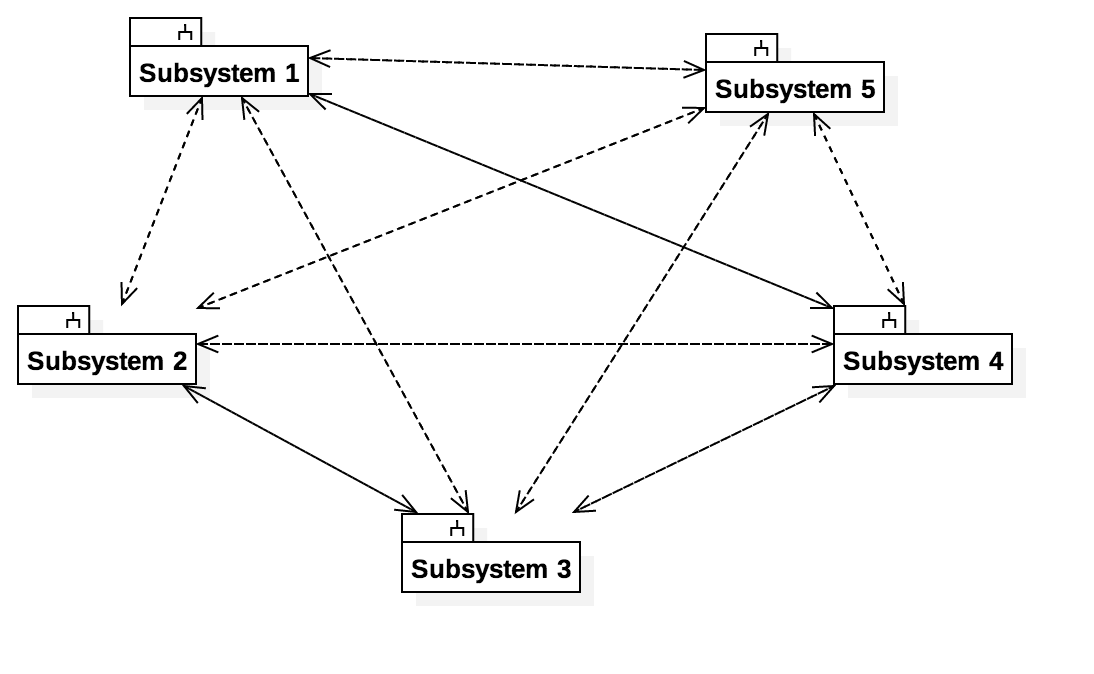
\includegraphics[width=15cm]{otros/UML/png/arquitectura_mala.png}
	\caption{Arquitectura con subsistemas interconectados directamente}
	\label{dia:arquitectura_mala}
\end{figure}

\bigskip

Aquí es donde entra la arquitectura basada en subsistemas conectados por el bus de mensajes que permite evitar las múltiples referencias y controlar con mucha más facilidad las comunicaciones dentro de la aplicación. En la figura \ref{dia:arquitectura_general} se observa la diferencia en términos de simplicidad y orden.

\bigskip

\begin{figure}
	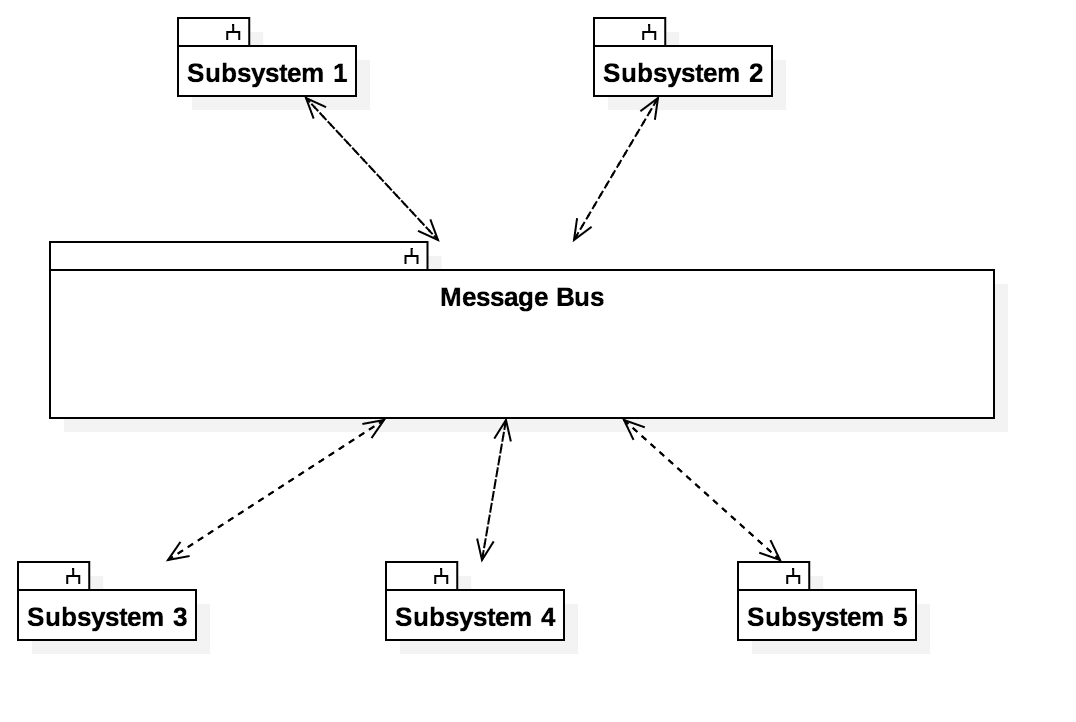
\includegraphics[width=15cm]{otros/UML/png/arquitectura_general.png}
	\caption{Arquitectura con subsistemas interconectados mediante bus de mensajes}
	\label{dia:arquitectura_general}
\end{figure}

\bigskip

De hecho, sobre la arquitectura general mostrada en la figura \ref{dia:arquitectura_general} se harán una serie de modificaciones de forma que todos los subsistemas sean totalmente transparentes a ojos del bus de mensajes. Para ello se hará que los mismos hereden de lo que llamaremos un \textit{Bus Node} o nodo del bus. La forma que tendría esta arquitectura de forma genérica es la mostrara en la figura \ref{dia:actual_arquitecture}

\bigskip

\begin{figure}
	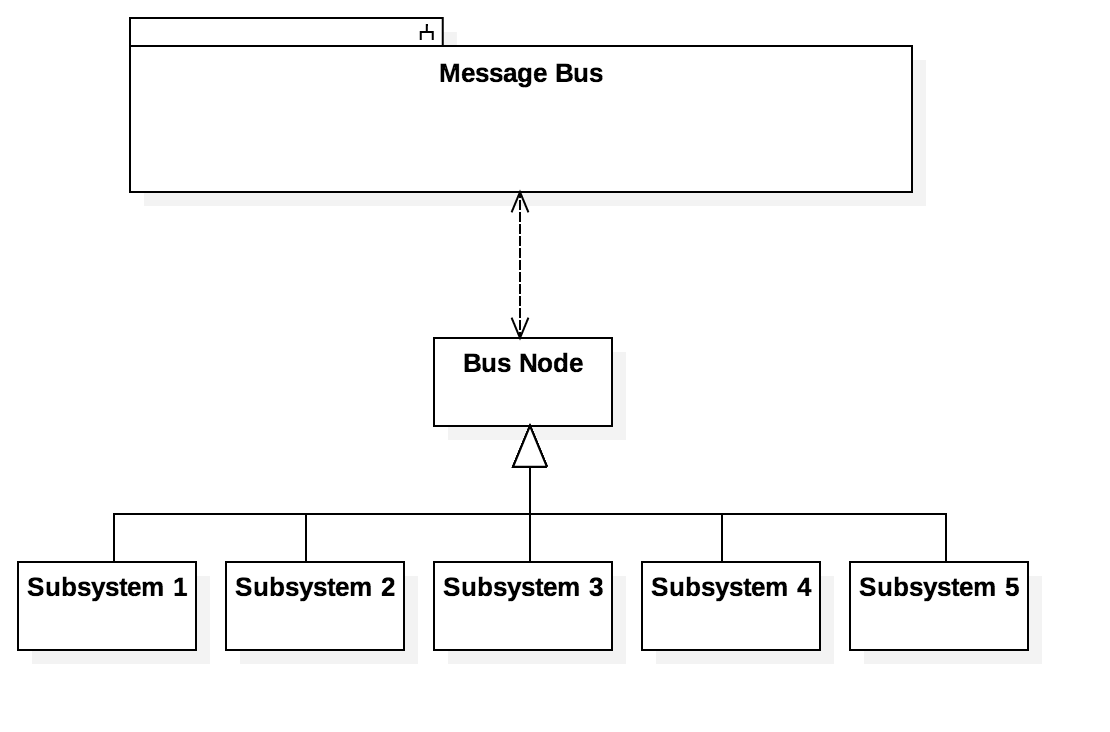
\includegraphics[width=15cm]{otros/UML/png/actual_arquitecture.png}
	\caption{Arquitectura con Bus Node}
	\label{dia:actual_arquitecture}
\end{figure}

\bigskip

Sobre esta arquitectura general se realizará una modificación relacionada con el requisito no funcional RNF-4 para facilitar los procesos de depuración de errores. Dado que todos los mensajes pasarán por el bus de mensajes se podrá hacer que los mismos sean mostrados en la consola interna de la aplicación o incluso introducir mensajes en forma de comandos en dicha consola. Para hacer esto posible se necesitará tratar de modo especial la consola como subsistema de forma que la arquitectura final será la que se puede ver en la figura \ref{dia:arquitectura_final}.

\bigskip

\begin{figure}
	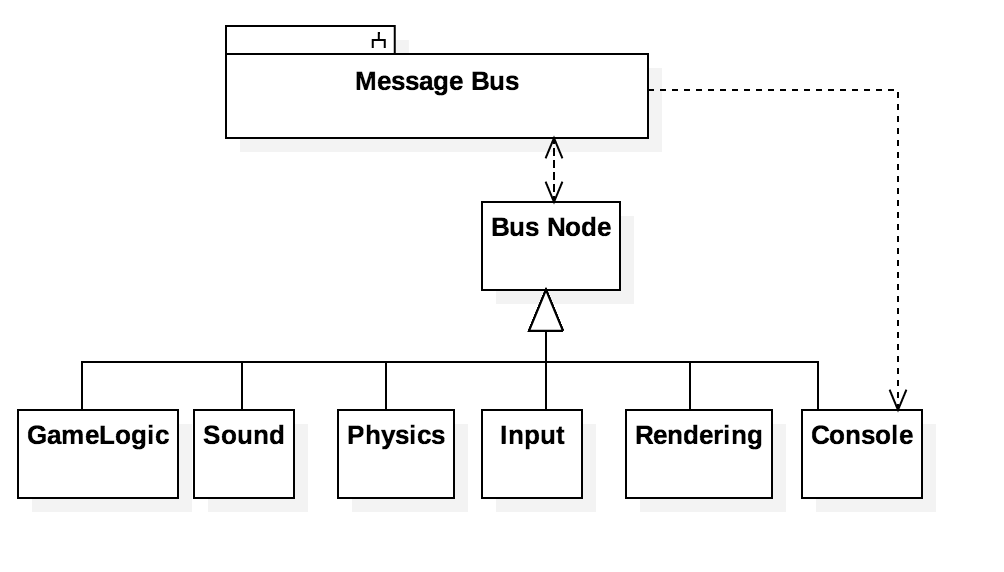
\includegraphics[width=15cm]{otros/UML/png/final_arq.png}
	\caption{Arquitectura final}
	\label{dia:arquitectura_final}
\end{figure}

\bigskip

También podemos observar en la figura \ref{dia:arquitectura_final} el componente que representa la lógica del juego es la que ocasionará que se ejecuten las diferentes funcionalidades de una forma u otra. Como \textit{GameLogic} se entiende a todas las clases dedicadas a definir los datos y comportamiento del videojuego en un determinado estado, por ejemplo, la lógica de un menú contendrá las opciones disponibles con la acción que corresponde a cada una de ellas, además tendrá la funcionalidad de cambiar entre las mismas y seleccionar la que se desee.

\bigskip

\subsection{Subsistemas propios del motor}

En relación a la figura \ref{dia:arquitectura_final} se dedicará este apartado a explicar la función general de cada uno de los subsistemas que no componen la lógica de la aplicación o \textit{GameLogic}.

\begin{itemize}
	\item \textbf{\textit{Sound} o Sonido}: Será el subsistema encargado de reproducir cualquier tipo de sonido que necesite la aplicación, desde pequeñas indicaciones que confirman que se ha cambiado de opción en el menú hasta el sonido de realizar un ataque, incluyendo música si se fuera a añadir.
	\item \textbf{\textit{Physics} o Físicas }: Será el subsistema encargado de lidiar con todas las funcionalidades relacionadas con la simulación de físicas en la aplicación. Esto puede incluir detectar colisiones contra muros y evitar que se puedan atravesar o detectar cuando un ataque realizado por un personaje ha alcanzado al otro o no.
	\item \textbf{\textit{Input} o Entrada}: Será el subsistema que recibirá todas las entradas realizadas por el usuario, desde teclas pulsadas hasta movimientos de un joystick, para luego enviárselas a los otros subsistemas para que gestionen si deben ejecutar algún proceso.
	\item \textbf{\textit{Rendering} o Renderizado}: Será el subsistema encargado de mostrar cualquier tipo de gráficos por pantalla. Necesitará gestionar la ventana y todas sus acciones (cambiar el tamaño, cerrarla, etc.). Además contendrá la funcionalidad de mostrar las animaciones realizadas, texto, efectos, etc.
	\item \textbf{\textit{Console} o Consola}: Será el subsistema utilizado para ver los mensajes importantes de la aplicación así como enviar mensajes en forma de comandos introducidos en tiempo de ejecución. Será la interfaz que el usuario tendrá para introducir mensajes directamente en el bus de mensajes.
\end{itemize}
  

\section{Herramientas de diseño}

Los modelos formales mostrados en esta memoria utilizan UML o \textit{Unified Modeling Language}. En términos de lenguajes de modelado para software este es sin duda el estándar más expandido, soportado además por el OMG\footnote{\textit{Object Management Group}: Consorcio dedicado a establecer y gestionar estándares relacionados con el paradigma de la orientación a objetos}.

\bigskip

Pese a que el lenguaje completo en su versión 2.5 ofrezca 14 tipos de diagramas específicos, en esta memoria se han utilizado solamente 4, siendo los mismos:

\begin{itemize}
	\item \textbf{Diagrama de casos de uso}: Dedicado a modelar el comportamiento del sistema ante los actores que interactúan con él.
	\item \textbf{Diagrama de paquetes}: Utilizado para mostrar los subsistemas y componentes genéricos de la aplicación.
	\item \textbf{Diagrama de clases}: Usados para definir y especificar las diferentes clases de cada subsistema y las relaciones entre las mismas.
	\item \textbf{Diagrama de secuencia}: Que modelan los casos de uso definidos en términos de la interacción entre objetos de la aplicación.
\end{itemize}

\subsection{Herramientas software}

Relacionado con el diseño solo se ha utilizado una aplicación concreta siendo la misma el \textit{StarUML 2.8}\footnote{\url{http://staruml.io/}}. La elección surgió a raíz de históricamente que ha sido la seleccionada para modelar durante la carrera y no se han experimentado deficiencias en términos de funcionalidades que implicaran tener que buscar un sustituto.

\subsection{Patrones de diseño}

Al trabajar con el paradigma de orientación a objetos es muy común que, si se diseña o programa sin prestar atención a las necesidades de la aplicación y sin considerar lecciones aprendidas anteriormente, se llegue a una situación en la cual se ha desarrollado una solución extremadamente compleja para un problema relativamente simple. A muy alto nivel, las lecciones aprendidas por parte de toda la comunidad de programadores y diseñadores se representan en forma de \textbf{patrones de diseño}.

\bigskip

Un patrón de diseño representa una solución a un problema común y genérico que ha sido generada y probada a partir de su uso continuado por parte de la comunidad. Lo que aporta esto es la flexibilidad de aplicar soluciones con la seguridad de estar utilizando modelos simples y potentes que no generarán errores en el diseño si se usan correctamente. Además, su implementación se hace significativamente más sencilla ya que la documentación y recursos disponibles para aprender a codificarlos está muy extendida.

\bigskip

En las siguientes secciones de este apartado se muestran los patrones utilizados de forma consciente en la aplicación ya que es relativamente común que debido a la práctica se lleguen a diseños que contienen patrones sin haberse propuesto implementarlos.

\bigskip

\subsubsection{Patrón \textit{Strategy}}

Para la implementación de comportamientos diferentes del enemigo nos será de mucha utilidad el patrón \textit{Strategy}  ya que el mismo está enfocado a cambiar los algoritmos que definen el comportamiento de un objeto de forma dinámica. De esta forma se puede cambiar fácilmente entre el enemigo controlado por el agente o el controlado por reglas siendo esto transparente al personaje que está siendo controlado.

\bigskip

Este patrón aporta una serie de ventajas relevantes para nuestro caso que son las siguientes:

\begin{itemize}
	\item No se tiene que agregar el código de los algoritmos al cliente (personaje) ya que el mismo puede ser muy complejo.
	\item El cliente no necesita todos los algoritmos en todas las situaciones por lo que evitamos que sea él el que los almacene.
	\item Si existen varios clientes que utilicen los mismos algoritmos se evita duplicar el código.
\end{itemize}

\bigskip

En la figura \ref{pat:strategy} se observa una definición genérica del patrón donde las diferentes partes son:

\begin{itemize}
	\item \textbf{\textit{Context}}: La clase que contendrá a la estrategia sea cual sea la misma. Esto puede ser el propio cliente o puede estar contenida en él.
	\item \textbf{\textit{Strategy}}: Clase abstracta que representa a una estrategia genérica, por si misma no contiene comportamiento alguno.
	\item \textbf{\textit{ConcreteStrategy}}: Clase que implementa cada uno de los diferentes comportamientos entre los que se puede cambiar.
\end{itemize}

\bigskip

\begin{figure}
	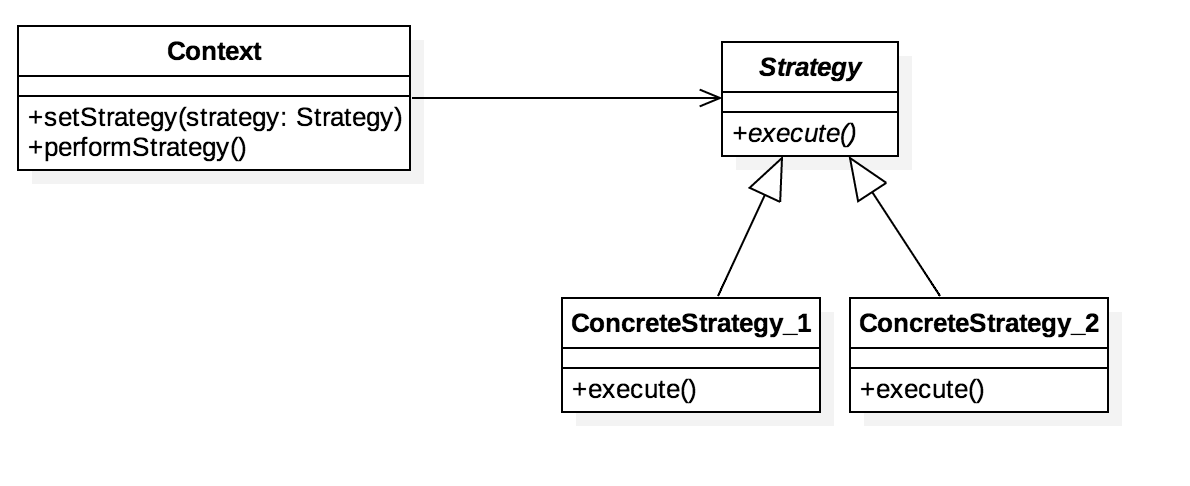
\includegraphics[width=15cm]{otros/UML/png/strategy.png}
	\caption{Patrón \textit{Strategy}}
	\label{pat:strategy}
\end{figure}


\subsubsection{Patrón \textit{Singleton}}

A la hora de requerir que solo exista una instancia de un componente concreto en una ejecución del programa el patrón a utilizar es el conocido como \textit{Singleton}. Este patrón permite además hacer que ese componente sea accesible por cualquier otro con facilidad, algo comúnmente necesario en videojuegos ya que hay entidades como gestores de recursos, relojes o sistemas de colisiones que deben ser comunes y únicos.

\bigskip

Estas dos ventajas comentadas son las que han decantado la balanza a favor de su elección. Sin embargo se debe tener mucho cuidado con el uso de este patrón ya que puede suponer una refactorización de código muy importante si luego se decide que el objeto no debe de tener acceso global o que se necesitan varias instancias del mismo.

\bigskip

\begin{figure}
	\centerline{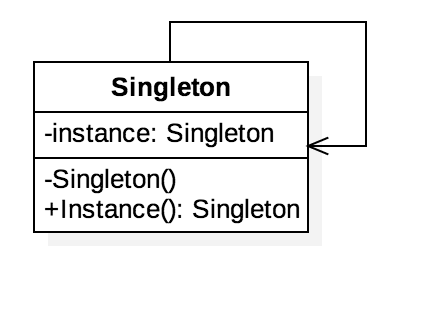
\includegraphics[width=5cm]{otros/UML/png/singleton.png}}
	\caption{Patrón \textit{Singleton}}
	\label{pat:singleton}
\end{figure}

\bigskip

En la figura \ref{pat:singleton} podemos ver el único componente que conforma el patrón. Esta clase tiene un método \textit{Instance()} que permite acceder a la única instancia que existe. Dicha instancia o \textit{instance} es privada, de la misma que el constructor \textit{Singleton()} para evitar así que se creen nuevos objetos desde fuera.


\subsubsection{Patrón \textit{Decorator}}

Cuando se necesita extender la funcionalidad de un objeto de forma dinámica el patrón más comúnmente usado es el conocido como \textit{Decorator}. El mismo permite agregar componentes a un objeto de forma que los mismos puedan contener operaciones o estado adicionales. En el contexto de un videojuego suele ser necesario que la escena en la que se trabaje y los objetos que están en ella se puedan gestionar de forma dinámica. Se explicará más en detalle en el apartado de diseño e implementación.

\bigskip

\begin{figure}
	\centerline{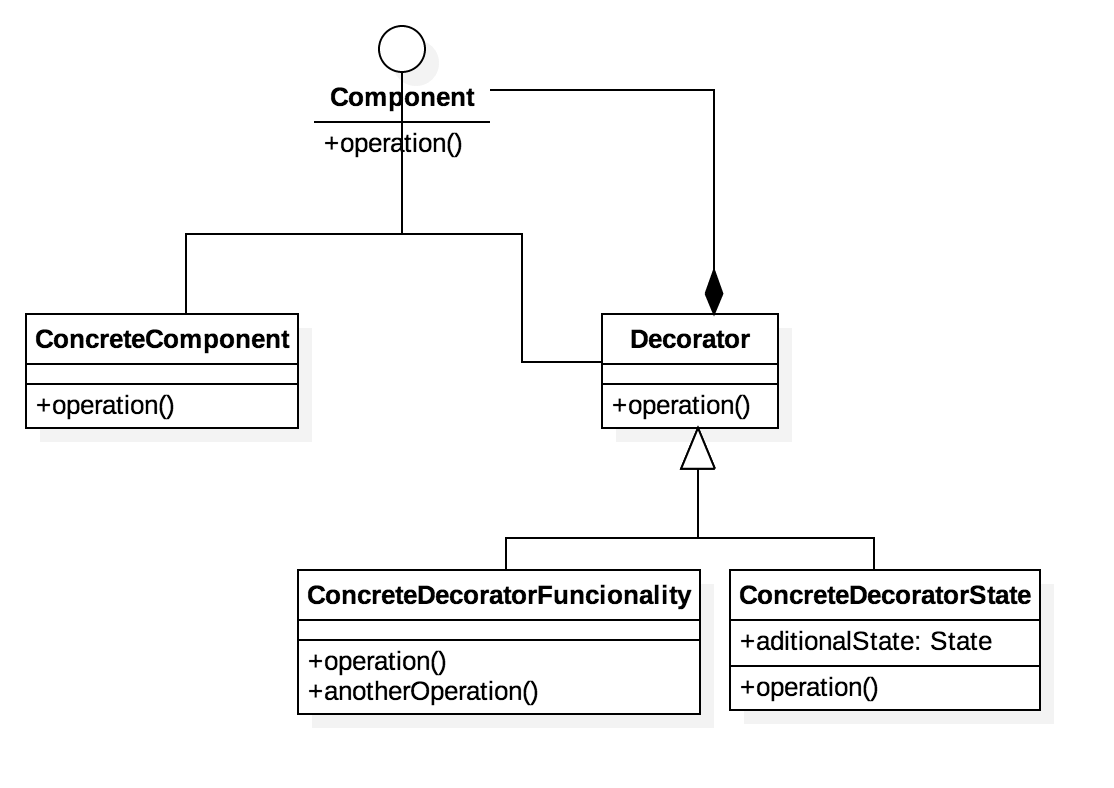
\includegraphics[width=12cm]{otros/UML/png/decorator.png}}
	\caption{Patrón \textit{Decorator}}
	\label{pat:decorator}
\end{figure}

\bigskip

En la figura \ref{pat:decorator} se ven los diferentes componentes que cuentan con las siguientes responsabilidades:

\begin{itemize}
	\item \textbf{\textit{Component}}: Interfaz para los objetos que pueden recibir nuevas responsabilidades dinámicamente.
	\item \textbf{\textit{ConcreteComponent}}: Objeto que puede recibir responsabilidades adicionales de forma dinámica.
	\item \textbf{\textit{Decorator}}: Referencia al objeto componente definiendo la interfaz que se ajusta a la interfaz del componente.
	\item \textbf{\textit{ConcreteDecorator}}: Extienden el componente añadiendo funcionalidad y/o estado.
\end{itemize}

\subsubsection{Patrón Publica-Subscribe o \textit{PubSub}}

El patrón Publica-Subscribe se utiliza cuando es necesario que diversos objetos reciban ciertos mensajes en los que pueden estar interesados mientras otros son los encargados de generar dichos mensajes. Esto se dá en el caso del  bus de mensajes ya que los diferentes subsistemas están interesados en recibir los mensajes relevantes para ellos.

\bigskip

\begin{figure}
	\centerline{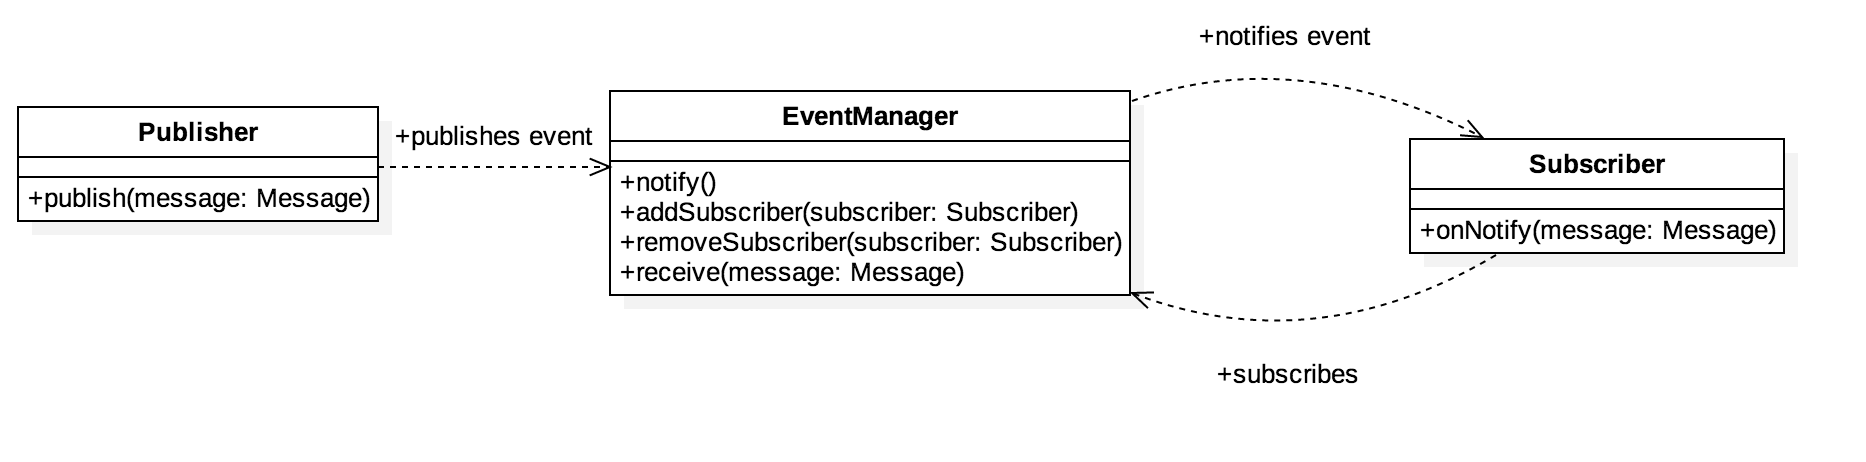
\includegraphics[width=18cm]{otros/UML/png/pubsub.png}}
	\caption{Patrón Publica-Subscribe o \textit{PubSub}}
		\label{pat:pubsub}
\end{figure}

\bigskip
 
En la figura \ref{pat:pubsub} se pueden observar los componentes del patrón que realizan las siguientes funciones:

\begin{itemize}
	\item \textbf{\textit{Publisher}}: Objeto que genera los mensajes y los envía al \textit{EventManager}.
	\item \textbf{\textit{EventManager}}: Objeto que recibe los mensajes y los distribuye a los subscriptores, además permite agregar o quitar subscriptores de forma dinámica.
	\item \textbf{\textit{Subscriber}}: Objeto encargado de subscribirse que luego recibirá los mensajes por parte del \textit{EventManager}.
\end{itemize}

\bigskip

Tenemos que comentar que en la aplicación, como se ve en el apartado de diseño, se realizará una aproximación ligeramente diferente en la cual todos los subsistemas publican y reciben mensajes. Estas dos responsabilidades estarán asociadas al \textit{BusNode} que es el que se conectará con el bus de mensajes que representa al \textit{EventManager}.


\section{Herramientas de desarrollo}

La elección de las herramientas de desarrollo utilizadas en este proyecto ha estado significativamente influenciada por el conocimiento previo que se tenía de las mismas. Esta práctica es habitual en todos los proyectos pero se vuelve más necesaria aún cuando el tiempo disponible para realizar el proyecto está limitado.

\bigskip

En este sentido, prácticamente siempre que se pudo elegir una herramienta conocida para realizar alguna tarea se ha escogido. Dicho esto, el entorno de desarrollo a rasgos muy generales que se ha utilizado está compuesto por las siguientes herramientas:

\bigskip

\begin{itemize}
	\item \textbf{Sistema operativo}: macOS Sierra 10.12.5
	\item \textbf{Compilador}: clang 802.0.42 (basado en Apple LLVM 8.1.0)
\end{itemize}

\bigskip

El entorno es relativamente  corto y fácil de describir dada la ausencia de bases de datos o frameworks que corran por encima del lenguaje utilizado. Pese a que en la lista anterior solo se mencionen el sistema y compilador utilizados, se entrará en detalle sobre las herramientas específicas dedicadas a la elaboración de la documentación, el desarrollo del código, las tecnologías elegidas y las librerías utilizadas.

\subsection{Realización de la documentación}

Para generar la documentación del proyecto y, por lo tanto, esta misma memoria se han utilizado las siguientes herramientas:

\begin{itemize}
	\item \textbf{TeXstudio\footnote{\url{http://www.texstudio.org/}}}: La elección de este editor para archivos .tex se ha escogido dado su amplio uso en la comunidad, la cantidad y calidad de la documentación del mismo y el hecho de que es soportado en todos los sistemas operativos importantes, lo que reduce el riesgo de tener que utilizar otra herramienta si ocurren problemas con el equipo de desarrollo.
	\item \textbf{Microsoft Project 2013}: Gracias a las versiones de prueba que ofrece Microsoft para este software se ha podido utilizar esta herramienta. Teniendo la opción de elegir entre las diferentes opciones orientadas a la gestión de proyectos la mejor sin duda es Project. Aporta muchas más facilidades y posibilidades que los competidores y es el estándar de facto. Además, si las versiones de prueba dejan de estar disponibles, muchas de las otras herramientas soportan la importación de proyectos de Microsoft Project, posibilitando así continuar con el proyecto.
	\item \textbf{StarUML 2.8}: Usado tanto para elaborar los diagramas como para exportarlos a imágenes integrables en la documentación. Como 
\end{itemize}


\subsection{Desarrollo}

Las herramientas que han sido necesarian para llevar a cabo la implementación de la aplicación han sido las siguientes:

\begin{itemize}
	\item Motor \textbf{Unity 5}: Se escogió como herramienta principal para desarrollar la aplicación hasta que se descubrieron las limitaciones mencionadas en la acción correctiva AC-1. La elección inicial estaba fundamentada en las facilidades que otorga para implementar aplicaciones de este tipo y la consecuente velocidad a la hora de obtener versiones funcionales rápidamente.
	\item IDE \textbf{MonoDevelop}: Necesario para trabajar con el código en C\# que utiliza Unity en macOS. Pese a que sea un IDE simplemente se utilizaba para la edición de código dadas las facilidades a la hora de detectar errores en el mismo.
	\item IDE \textbf{Xcode 8.3.3}: Al estar estrechamente integrado con el sistema de Apple nos permite realizar todo el desarrollo en un mismo entorno. Automáticamente busca y utiliza las herramientas por defecto a la hora de detectar errores en el código, compilar, depurar y empaquetar la aplicación. Además integra un potente \textit{profiler} que ayuda a detectar los cuellos de botella de la aplicación, algo muy importante en situaciones como esta en la que el rendimiento es importante.
	\item Compilador \textbf{clang-802.0.42 basado en Apple LLVM 8.1.0}: La elección de este compilador era clara, además de soportar las especificaciones de C++ necesarias (completamente hasta C++14) también puede compilar código escrito en Objective C, ya que se ha requerido para una pequeña parte relacionada con el empaquetado de la aplicación. Este compilador es automáticamente utilizado por Xcode por lo que a ojos del usuario es completamente transparente.
\end{itemize}

\subsection{Tecnologías}

Las tecnologías que se incluyen en este apartado están compuestas por los diferentes lenguajes de programación escogidos para cada una de las partes, así como de cualquier otro tipo de lenguaje que se haya tenido que utilizar.

\begin{itemize}
	\item \textbf{C\#}: Elegido porque es el lenguaje que utiliza Unity para correr los diferentes archivos o \textit{scripts} que definen el comportamiento de los objetos del juego.
	\item \textbf{C++}: Dada la relativa experiencia que el desarrollador tenía en este lenguaje se consideró el mismo una buena opción para el proyecto. Más incluso cuando se consideró que el rendimiento era importante dado que la ausencia de un \textit{runtime} encargado de correr nuestro código, realizar recolección de basuras, etc podía ser catastrófico a la hora de conseguir la velocidad de simulación deseada. Además, en términos de lenguajes compilados a bajo nivel C++ es el que más se ajustaba al paradigma orientado a objetos.
	\item \textbf{Objective-C}: Extensión de C orientada a objetos similar a C++ pero utilizado principalmente en sistemas Apple. Nos ha permitido encapsular todos los archivos y recursos de la aplicación en un mismo ejecutable, haciendo el producto final extremadamente portable en todos los sistemas macOS. 
	\item \textbf{JSON}: Formato de texto orientado a la transmisión y representación de datos de forma ligera. Se ha utilizado para escribir los datos referentes a las animaciones para así saber que imagen se debe mostrar, en que orden y durante cuanto tiempo. 
\end{itemize}

\subsection{Librerías}

Finalmente, las librerías utilizadas simplemente se referirán a las que son llamadas desde el código C++ pues los otros lenguajes no requerían extensión alguna para realizar las funcionalidades que se implementaron con ellos.

\begin{itemize}
	\item \textbf{Biblioteca estándar de C++}: Básica a la hora de trabajar con C++ ya que soporta los contenedores genéricos y funcionalidades asociadas más utilizados en el lenguaje a la vez que completa las características del mismo al soportar funcionalidades en entrada y salida a archivos o salida estándar. 
	\item \textbf{SFML}: Librería a bajo nivel que sirve como interfaz sobre OpenGL. Gestiona la creación de ventanas en el sistema operativo que se requiera y ofrece funcionalidades útiles a la hora de mostrar por pantalla, reproducir sonidos, etc.
	\item \textbf{json.h}: Librería en formato de cabecera única que sirve para facilitar la lectura y escritura de archivos json. Disponible en GitHub\footnote{\url{https://github.com/sheredom/json.h}} en la cuenta de su creador, \textit{sheredom}, el cual la proporciona sin requerir ningún tipo de licencia.
	\item \textbf{Boost}: Conjunto de bibliotecas de software libre enfocadas a extender al lenguaje C++ con funcionalidades comúnmente necesitadas como realización de operaciones algebraicas complejas, procesamiento de imágenes, expresiones regulares o nuevos tipos de datos.
\end{itemize}

